%%%Preamble
\documentclass[12pt]{article}
\usepackage{epsfig, amsfonts, cite, amssymb}
\usepackage{subfigure}
\usepackage{array}
\usepackage{float}
\usepackage{enumitem}
\usepackage{indentfirst}
\usepackage{boldline}
\usepackage[usenames,dvipsnames,svgnames,table]{xcolor}
\usepackage{amsmath}
\usepackage[a4paper]{geometry}
\geometry{top=1.in, bottom=1in, left=1in, right=1in}

%%% Use these when running Text Verifications
%\usepackage[T1]{fontenc}        
%\usepackage[utf8]{inputenc}     
%\usepackage[adobe-utopia]{mathdesign}
%\usepackage{printlen}

\voffset=0in \hoffset=0in \textwidth=6.3in \textheight=8.3in
\setlength{\oddsidemargin}{0in} \setlength{\textwidth}{6 in}

\newcolumntype{C}[1]{>{\centering\arraybackslash}m{#1}}
\newcolumntype{M}[1]{>{\arraybackslash}m{#1}}
\newcolumntype{N}{@{}m{0pt}@{}}

\thispagestyle{empty}

\begin{document}

%%%Header
\begin{figure*}[htb]
\subfigure{
\includegraphics[width=2.5in]{wne.eps} }
\hfil \hspace{.5in}
\subfigure{
\includegraphics[width=2.5in]{department.eps} }
\end{figure*}



%%%Cover Page
\begin{center}
{\Large {\bf CPE 462/562 VHDL: Simulation \& Synthesis}}\\
\vspace{0.2in}
Final Project - Fall 2017 \\ 
\vspace{0.2in}
{\Large{Vending Machine Design, Verification, and Implementation}} \\
\vspace{0.2in}
Katelyn Charbonneau \\
Email: kc325844@wne.edu\\
Date: 12/8/2017
\end{center}


  
\begin{table}[!h]
\centering
%\ \begin{tabular}{| >{\arraybackslash}m{4in}{1in} | >{\centering\arraybackslash}m{1in} | }
\begin{tabular}{|M{10cm}|C{3cm}|N}
  \hline
  % after \\: \hline or \cline{col1-col2} \cline{col3-col4} ...
  \textbf{Tasks} & \textbf{Grades} \\ [20pt]
  \hline
Select product, choose to buy the product, and display product name and price (10') & \\ [30pt]

  \hline

  Cancel transaction, display returned amount, and show idle state (20') & \\ [30pt]

  \hline
  
  Insert coins, display the left amount for purchase on SSD, and reject invalid coins (40') & \\ [30pt]

  \hline

  Deliver product, and display change on SSD (20') & \\ [30pt]
  
  \hline
 
 Report (10') & \\ [30pt]
 
  \hline
    \hline

 Total (100') & \\ [30pt]
  
  \hline
\end{tabular}
%\caption{}
%\label{table_p1}
\end{table}

%%%Text Verifications
%This text is \fontname\font\ with font size \csname f@size\endcsname{}
%and \verb|\baselineskip| =~\the\baselineskip =~\uselengthunit{mm}\printlength{\baselineskip}.

%%% END of Cover Page
\newpage

\section{Objective} \label{sec:obj}
The objectives of the project are to design and implement a simple vending machine; be able to write VHDL code to design said system using a state machine; and implement the system on the Altera DE-115 FPGA.

\section{Design Procedure} \label{sec:desproc}
The first step in designing a system using state machines is to draw a state diagram, which is shown in Figure \ref{fig:toplevel}.

\begin{figure}[!h]
\setlength{\belowcaptionskip}{-10pt}
\begin{center}
\includegraphics[scale=0.6]{StateDiagram.png}
\caption{Vending machine state diagram}
\label{fig:toplevel}
\end{center}
\end{figure}

Development of the VHDL code went state-by-state for simplicity.  After the behavior of each state was defined, the code for that state was programmed onto the board and tested.\par
The first state that was designed was the Idle state.  For this state, a record type was declared to contain product information for each of the products.  The information included was the product code (two bits standard logic), product abbreviation (character), and price.  While records were not covered in class, previous familiarity with similar techniques such as dictionaries from the Python language made using one simple.  Using the record allowed the Idle state to be written in much more concise, readable code.\par
The idle state displays dashes (-) on all of the seven-segment displays (SSDs) used in the project (Hex 5, 2, 1, and 0).  When a user presses the product choose button (Key 3), the product abbreviation and price will take on the value of whichever product was selected with the switches (Switch 17 and 16), then transitions to the UserTransaction state.\par
The UserTransaction state is the next that was developed.  It also contains most of the logic that dictates the behavior of the system.  For this system, a number of signals had to be declared to handle the operations required.  One signal is simply the price of the selected product.  Because it could be any of the four products offered, it had to be able to be changed; although it is not altered within this state (it is set in the Idle state).  The second signal is the amount of money that is the customer has inserted.  The third is a catch-all signal that is ultimately passed to the output ports of the system; this signal takes on a value of some function of the previous two signals and itself, depending.  When the user inserts a coin, the paid amount increases by that coin's value, and the display on the SSDs decreases by that coin's value.  When the paid amount is greater or equal to the cost amount, the state transition to Delivery occurs.  If the user presses the cancel button (Key 0), the state transition to the Cancel state occurs.\par
The Cancel state is simple: it displays on the SSDs the amount of money to be returned.  This value is equal to the value of the paid amount signal.  After 5 seconds, the system will transition to the Idle state.  The Delivery state is also simple: it displays on the SSDs the amount of change to be returned.  This value is equal to the value of the paid amount minus cost amount.  The delivery LED will also blink 5 times, after which the system will transition to the Idle state.\par
For simplicity, the values of the aforementioned signals involving money are all 3-digit (000 to 999) integer types.  A component was written to "index" into these values and separate them into 3 1-digit integer types.  This was so they could easily be used for the SSD function.  The component uses the MOD operator and the divide operator (which floors the result) to do this.  In addition, the frequently used push button debouncer component was used for the buttons in this project.

\section{Simulation Results} \label{simresults}

\begin{figure}[H]
\begin{center}
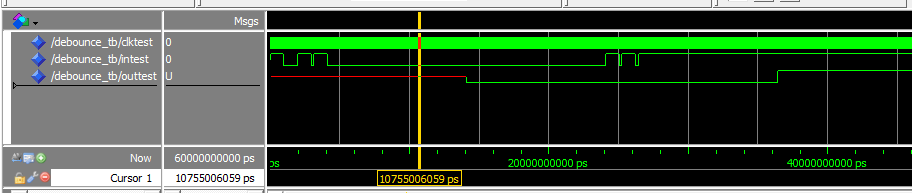
\includegraphics[scale=0.6]{debounce_sim.png}
\caption{Showing debouncing program works with simulated bouncy input}
\label{fig:simdb}
\end{center}
\end{figure}

\newpage

\section{Demonstration on FPGA} \label{demo}
The design was synthesized onto the Altera Cyclone IV E DE2-115F29C7 FPGA.
\begin{itemize}
\item User Controls:
	\begin{itemize}
	\item Product Select: Switches 17 and 16
	\item Product Choose: Key 3
	\item Coin Select: Switches 1 and 0
	\item Coin Choose: Key 2
	\item Cancel: Key 0
	\end{itemize}
\item Output Displays:
	\begin{itemize}
	\item Product Abbreviation: Hex 5
	\item Main Display: Hex 2, 1, and 0
	\item Delivery Alert: Green LED 8 (LEDG8)
	\end{itemize}
\end{itemize}

\begin{figure}[H]
\begin{center}
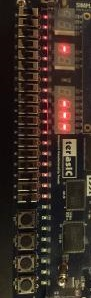
\includegraphics[scale=1.0,angle=90]{----.png}
\caption{Display in Idle state}
\label{fig:board1}
\end{center}
\end{figure}

\begin{figure}[H]
\begin{center}
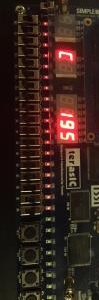
\includegraphics[scale=1.0,angle=90]{C195.png}
\caption{Display after choosing Coffee}
\label{fig:board2}
\end{center}
\end{figure}

\begin{figure}[H]
\begin{center}
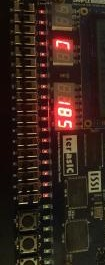
\includegraphics[scale=1.0,angle=90]{C185.png}
\caption{Inserted a dime}
\label{fig:board3}
\end{center}
\end{figure}

\begin{figure}[H]
\begin{center}
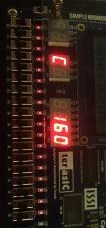
\includegraphics[scale=1.0,angle=90]{C160.png}
\caption{Inserted a quarter}
\label{fig:board4}
\end{center}
\end{figure}

\begin{figure}[H]
\begin{center}
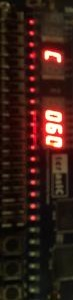
\includegraphics[scale=1.0,angle=90]{C60.png}
\caption{Inserted a dollar}
\label{fig:board5}
\end{center}
\end{figure}

\begin{figure}[H]
\begin{center}
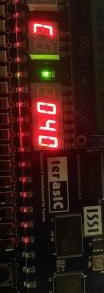
\includegraphics[scale=1.0,angle=90]{C40Delivery.png}
\caption{Inserted another dollar; delivery in progress; displaying change}
\label{fig:board6}
\end{center}
\end{figure}

\begin{figure}[H]
\begin{center}
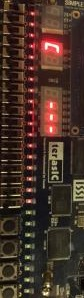
\includegraphics[scale=1.0,angle=90]{C---.png}
\caption{Inserted an invalid coin}
\label{fig:board7}
\end{center}
\end{figure}

\begin{figure}[H]
\begin{center}
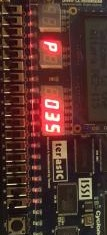
\includegraphics[scale=1.0,angle=90]{P35.png}
\caption{Inserted a quarter and dime; canceled; displaying return change}
\label{fig:board8}
\end{center}
\end{figure}

\newpage

\section{Conlusion} \label{cncl}
The project simulated and synthesized correctly.  The code required sufficient knowledge of structural, concurrent, and sequential VHDL. A package was designed to compartmentalize the code to make it easier to read and debug.  Recently learned functions and procedures were used within this package, as well as components used and user-defined data types.  A current issue is that the product abbreviation SSD (Hex 5) currently displayed a dash in the Idle state.  A more user-friendly design would be to display the abbreviation before the product is selected; otherwise, the customer needs an external way to know which code goes with which product.  Other than that, the project was very cleanly and quickly developed.  A strong base of knowledge and practice with VHDL and understanding of hardware constraints has been achieved as a result of not only this project, but the entire course.  This knowledge could also serve as a jumping off point if another hardware description language, for example Verilog HDL, needs to be used in the future.

\end{document} 
